%! program = pdflatex

\documentclass[11pt,a4paper]{article}
\usepackage[a4paper, twoside=false, tmargin=2.5cm, bmargin=2.5cm, inner=2.5cm, outer=2.5cm]{geometry}
\usepackage[T1]{fontenc}
\usepackage[english]{babel}
\usepackage[english]{varioref}
\usepackage{changepage}
\usepackage{graphicx, float, caption, subfig, amsmath, amssymb, mathrsfs}


\title{Identity-Preserving Low-Resolution Face Recognition}
\author{Arina \textsc{Lozhkina}}

\makeatletter 
\AtBeginDocument{\markboth{\@author}{\@title}} 
\AtBeginDocument{\renewcommand{\labelitemi}{-}}

%%% BEGIN DOCUMENT
\begin{document}

%TITLE
\begin{titlepage}
\begin{center}

{\Large \textsc{Electrical and Electronics Engineering}}\\\medskip
{\Large \textsc{Semester Project}}\\\medskip
{\Large Master Semester 3 - Autumn 2022}\\\vspace{4cm}

{\Huge \@title}\\\vspace{4cm}

\begin{tabular}{ll}
{\Large \textit{Student:}}   & {\Large \@author} \\  & \\
{\Large \textit{Supervised by:}}
& {\Large Yuhang \textsc{Lu}}  \\ 
& {\Large Prof. Dr. Touradj \textsc{Ebrahimi}} 
\end{tabular}
\vspace{3.5cm}

{\Large \@date}\vspace{3cm}

{\Large \textsc{Multimedia Signal Processing Group}}\\\medskip
{\Large \textsc{EPFL}}\\\vspace{7mm}

\includegraphics[width=4cm]{EPFL_LOGO.png}

\end{center}
\end{titlepage}
%END TITLE

\newpage

\pagenumbering{roman}
\addcontentsline{toc}{section}{Abstract}

\begin{abstract}
Despite significant advances in high-resolution recognition, low-resolution facial recognition remains a challenge. Many methods have been proposed for its solution, which can be divided by 2 categories: super resolution methods and resolution-invariant feature extraction. In this work the focus is on the second one. 

In the project the problem of low resolution face recognition is studied including methods of solving cross-resolution and low-resolution face recognition problem, the pipeline of face recognition based on deep learning and the low resolution datasets and their evaluation protocols. 

The high resolution facial recognition methods are implemented: CosFace, SphereFace and ArcFace. They are also adapted for low resolution face recognition problem using the Cross Resolution Batch training. Also the finetuning methods: Octuplet Loss and DeriveNet are implemented.  The implementation of face recognition pipeline based on the existing implementation is included. All methods are tested and compared using low resolution face images. 

Three low resolution datasets: LFW, SCface, QMUL-SurvFace, and their evaluation protocols are studied and implemented. 

One of the modern directions is the application of adaptive margin function. The proposed methods are based on it, which adapt margins for images of different quality. The quality of the images is considered using the Laplacian operator. The proposed methods surpassed the state-of-the-art algorithm of Cross Resolution Face Recognition, AdaFace, when tested on low resolution images. 

\end{abstract}

\newpage

\tableofcontents

\newpage

\pagenumbering{arabic}

\setcounter{page}{1}

\section{Introduction}

With the development of deep neural network technologies, the solution to the problem of face recognition in images has reached 0.9981 based on the LFW \cite{lfw} testing of ArcFace \cite{arcface} training loss \cite{magface}. This was facilitated by the availability of computational resources for calculations \cite{Susceptibility}, extensive datasets for training \cite{celeb}, the general development of computer vision, which led to the formation of new architectures of models \cite{20},  loss functions \cite{26}, preprocessing algorithms \cite{aug} and  image transformation \cite{13}.

However, these algorithms were trained and tested on high quality images such as LFW \cite{lfw} and CelebMV1 \cite{celeb}. At the same time, testing pre-trained algorithms on datasets close to real images of surveillance cameras like SCface \cite{scface} showed a significant decrease in accuracy when solving the problem of verifying faces in an image \cite{3}.

The reasons for this problem are face recognition challenges, which include low resolution, changes in facial expression, lighting, makeup, the presence of a mask, etc. For the practical application of face recognition systems, robustness of face recognition is required in images obtained in unconstrained environments \cite{deepFaceRecognition}.

This work focuses on the study, implementation and analysis of low-resolution facial recognition algorithms. In addition, within the scope of the work, new possible approaches have been developed to address the problem of low-resolution facial recognition. The second section is devoted to related work, in which the pipeline algorithm of recognition of persons based on deep learning is considered. Then there are low-resolution face recognition challenges, including low-resolution images. The following are the developed methods of solving the problem of recognition in low resolution. At the end of the review the variants of  loss functions used to solve the problem of face recognition are considered. The next section focuses on the test datasets including  LFW\cite{lfw}, QMUL-SurvFace\cite{qmul}, SCface \cite{scface}  and their evaluation protocols. Section 4 describes the algorithms implemented within the scope, including the adaptation of high-resolution facial recognition algorithms and fine-tuning. The following are two proposed methods for solving the problem of recognition in low resolution. In the end, the values of accuracy obtained by testing all implemented algorithms in comparison with the state-of-the-art face recognition algorithm in the cross-resolution, AdaFace \cite{adaface}, are given. 

\section{Related Work}
\subsection{Deep Face Recognition}
In recent years, deep face recognition, rather than manual extraction of features, has been an active trend \cite{deepFaceRecognition}. In this approach, the recognition process includes 3 steps: image preprocessing, model training to form embeddings and recognition by matching vectors in feature space \cite{deepFaceRecognition}. The pipeline is presented at \ref{fig:pipeline}.

\begin{figure}[ht!]
    \centering
    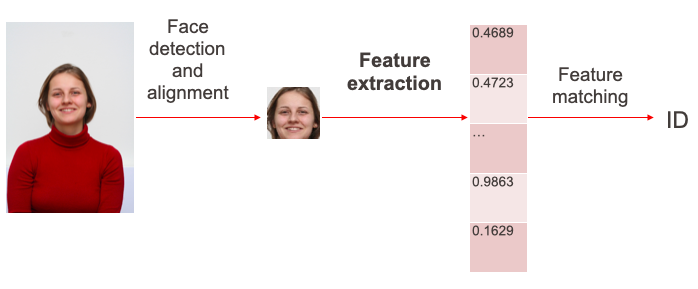
\includegraphics[width=\textwidth]{pipeline.png}
    \caption{Face Recognition Pipeline}
    \label{fig:pipeline}
\end{figure}

The intermediate step in some modern systems is the protection against face falsification by means of 3D masks, printing, etc. \cite{1} The result of model training for recognition is a feature vector of fixed length.

Preprocessing is needed to detect the face in the image and align it to the desired position. MTCNN Face Detection \cite{2} is used for face detection. MTCNN applies a cascade structure of deep convolutional networks that detect face position in a coarse-to-fine manner. Each model is trained to perform a separate task: classification, bounding box regression, and anchor point localization. Between steps, non-maximal suppression (NMS) is performed to filter out strongly overlapping candidates. 

\newpage

\subsection {Challenges} 
In unconstrained environments, face recognition is complicated by possible variations associated with changes in shooting conditions and facial variations, such as expressions of emotion, pose changes, occlusions such as masks and glasses, makeup, age changes, etc. When training a model on a dataset that includes uniform face images in full-face against a neutral background, its application to images in real-world face variations may be less effective \cite{3}.  

\begin{itemize}
\item{\bf{Poses}}

Camera placement affects the face pose of the resulting image. As a result of changes in shooting conditions, face images are no longer frontal, which leads to a deterioration in the performance of the recognition model \cite{4}. To assess the quality of recognition during changes in the pose of the face, the protocol P dataset Multi-PIE \cite{5}, which contains images of the face when the camera is rotated in 15 degree steps, is used. Frontal images are used as a template. 

\item{\bf{Partial occlusion}}

Partial occlusion is a common problem that involves partial concealment of the face with glasses, mask, and other elements, and affects face recognition performance \cite{6}. To evaluate the quality of recognition under partial occlusion, tests are performed on datasets such as AR \cite{7}, implementing performance evaluation based on expression, occlusion, illumination, and their combination protocols.  				
						
\item{\bf{Facial Expressions}}

Changing facial expressions leads to distortion of facial features \cite{8}, and as a consequence, a decrease in recognition quality. To evaluate the quality of recognition under conditions of facial expressions changes, the protocol E belonging to the test dataset Multi-PIE \cite{5} is used. Images with neutral facial expressions are used as a template image for each claimed identity.
\end{itemize}

\subsection{Low Resolution Face Recognition Methods}
One of the unresolved problems \cite{8} of face recognition is face recognition in low-resolution images. To solve this problem, 2 types of approaches have been identified: Transformation-Based and Non-transformation-based.

\subsubsection{Super Resolution}
When processing low-resolution images, one of the approaches is based on image transformation, which involves the transition to the space of high-resolution or super-resolution images \cite{9}. However, due to the addition of new information that does not belong to the low-resolution image, additional algorithms \cite{10, 11} are used to improve the accuracy of solving the identification problem, which optimize the transition to the super-resolution image space in order to preserve identity information. 

Generative Adversarial Networks, which also provide image synthesis for training, have become one distinct trend \cite{12}. GANs are also used to form a low-resolution training dataset, on the basis of which a feature space is identified separately for high- and low-resolution images, sharing information between networks \cite{13}. To improve accuracy, pre-training is used, while experimenting with loss functions, for example, using triplet loss \cite{14}. 

However GANs tend to produce over-smoothed images that doesn't permit to extract discriminative festures. To avoid this effect GPEN algorithm uses a method of 2 steps: learning a GAN to generate a high resolution image and embedding it into a deep neural network, and finetuning the GAN with LR face images. The results of GPEN \cite{gpen} algorithm are shown at the \ref{fig:super}. As the input the downsampled to (16, 16) and then interpolated to (112, 112) image is used. The results are compared to the original images. 

\begin{figure}[ht!]
    \centering
    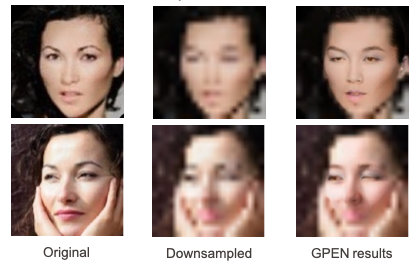
\includegraphics[width=\textwidth]{super_resolution.png}
    \caption{Results of GPEN}
    \label{fig:super}
\end{figure}


\subsubsection{Non-transformation-based approaches}
An alternative is to project an image of any resolution into a common feature space. For this, studies were carried out to develop the architecture of the model, the loss function, as well as the training method. With this approach, models may be trained on both high-resolution and low-resolution images, and the goal of training is to minimize the representation difference between them.

One proposed method is cross-resolution training based on a teacher-student distillation structure \cite{15}, in which the teacher processes high-resolution faces to form student distillation reference functions, and the student is trained to identify features similar to the teacher based on low-resolution data. 

A separate direction is multidimensional scaling, which processes low-resolution images using feature localization and translates high- and low-resolution pairs into a single feature space \cite{17}. To ensure the distinguishability of embeddings, discriminative multidimensional scaling is used \cite{16}.

Deep convolutional neural networks were taken as the basis for the development of model architects. Based on them, reliable partially connected networks were created \cite{18, 19}. Gated deep networks \cite{20} have been developed to process contextual information. Also, during their training, images of various resolutions were used \cite{21}. In addition, to identify resolution-resistant features, it is possible to use information from different layers of the neural network by combining their contextual functions \cite{22}.
To increase the speed of inference and model learning, distributed programming methods \cite{23}, as well as a two-threaded method of convolutional neural networks with selective knowledge distillation \cite{15}, were developed.

Modern methods \cite{25} also combine different approaches such as super-resolution, resolution matching, and multiscale template accumulation. It is also possible to adapt the loss functions, in this case the triplet loss, to obtain distinguishable representations in vector space for low-resolution images \cite{26} and add an additional term to the main loss function, necessary to minimize the distance between high-resolution image representations and its downsampled version \cite{27}.

\subsection{Loss Functions}
From the point of view of optimization, the task of face recognition corresponds to the transformation of an image into a vector representation in a feature space, where the distance corresponds to the measure of non-similarity of faces. 

\begin{itemize}
\item{\bf{Contrastive loss}}
Contrastive loss \cite{contrastiveLoss} involves measuring the degree of discrepancy between the obtained features for two images. If the images belong to the same class, then the discrepancy measure should be minimal, and vice versa. In addition, cosine distance can be used as a measure of discrepancy.
\item{\bf{Triplet loss}}
To obtain distinguishable features for classification, a triplet loss \cite{tripletLoss} function was developed. It is based on the concepts of an anchor -  a template image of the current personality, as well as a positive instance -  an image of the same personality, and a negative instance - an image of another personality. The purpose of formulating this function is to minimize the distance between feature vectors of one class and maximize with respect to features of other classes. This leads to the need for careful formation of the pairs contained in the training dataset.
\item{\bf{Center Loss}}
To better distinguish feature vectors, a loss function was introduced that calculates the centers for each class, Center Loss \cite{centerLoss}. Thus, the task of optimizing this component of the loss function is to minimize the distance between the center and the embedding. This loss can be added to another loss function such as Softmax \cite{softmax} to refine feature distribution.
\item{\bf{Octuplet Loss}}
One of the methods to improve resolution stability is Octuplet Loss \cite{26}. It is applied when fine-tuning FR models to solve the low resolution face recognition problem. This method is based on the application of Triplet Loss \cite{tripletLoss}, which has shown to be effective in detecting discriminative features. By applying Triplet Loss to images and their downsampled versions, it is possible to identify the relationship between them and improve performance in cross-resolution face recognition. \ref{fig:octuplet}  shows the Octuplet Loss \cite{26} algorithm.

\begin{figure}[ht!]
    \centering
    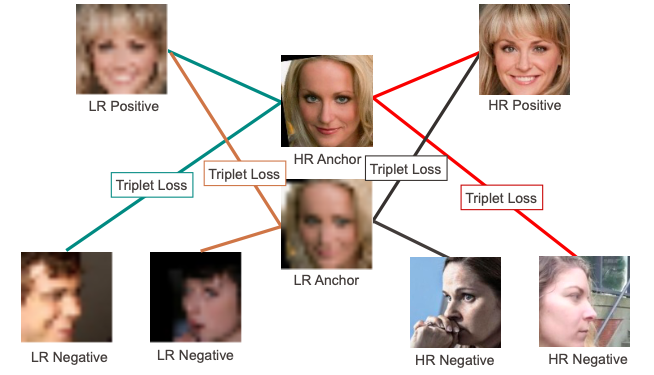
\includegraphics[width=\textwidth]{octuplet.png}
    \caption{Octuplet Loss}
    \label{fig:octuplet}
\end{figure}

\item{\bf{Softmax}}
Since face recognition is a classification problem, the softmax \cite{softmax}  was also tried in the formation of embeddings. Improving the accuracy of recognition during training based on softmax \cite{softmax} modifications has become one of the directions in face recognition.

\end{itemize}

\subsubsection{Softmax-based Loss Functions}
The softmax loss function can be improved by introducing a margin. The idea is that images of faces belonging to the same person should be closer to each other than images of any other classes, which in turn should be removed. Thus, the margin allows increasing intra-class compactness.
\begin{itemize}
\item{\bf{L-softmax}}
For the first time, the idea of margin was implemented in the loss function L-softmax \cite{Lsoftmax} by changing the cosine of the element angles. In addition, for the first time, softmax \cite{softmax} was formulated by presenting the scalar product of weights and features as the product of their norms by the cosine of the angle between them.
The idea is to position the embeddings on the hypersphere in such a way as to minimize the distance between the decision boundary and the class centers.
\item{\bf{A-softmax (SphereFace)}}
In A-softmax \cite{sphereface} the weight vector of each class is pre-normalized. In practice, optimization is carried out on a weighted sum of softmax and A-Softmax, the ratio of components of which changes with the number of iterations.
\item{\bf{NormFace}}
By modifying A-softmax \cite{sphereface}, the NormFace \cite{Normface} loss function was proposed, in which, in addition to the weights, the embedding vectors were also normalized. In addition, scaling of normalized vectors has been added.
\item{\bf{CosFace}}
By adding a margin outside the cosine,the loss function CosFace \cite{cosface} was formed. Also it normalizes the weights and the feature vector and introduces the scale parameter in order to reduce radial variations. The loss function is designed in such a way that a cosine margin permits to maximize the angular margin.
\item{\bf{ArcFace}}
In order to enhance the discriminative power of the algorithm the ArcFace \cite{arcface} was proposed. It is based on the idea that embedding features are arranged around their centers on the hypersphere, so to reinforce the intra-class compactness and inter-class discrepancy there is an additive margin penalty which is equal to the geodesic distance margin penalty in the normalized sphere. 
\item{\bf{P2SGrad}}
When training models with margin-based loss functions, it is necessary to set hyperparameters that can make the learning process unstable. To solve this problem, the loss function P2SGrad \cite{ps2grad} was designed, which formed the learning gradient adaptively.
\item{\bf{CurricularFace}}
This loss function \cite{curricularFace} introduces the idea of curriculum learning. In the initial stages, training is focused on simple instances. This is due to the small value of the margin. But in the course of learning, it increases in such a way that complex instances are also learned.
\item{\bf{UniformFace}}
UniformFace \cite{uniformface} was also based on the idea of ArcFace  \cite{arcface}that vector representations of faces lie on a hypersphere manifold. The problem it solves is above large margin losses do not take into account the distribution of classes in the training sample. To solve it, it was proposed to impose a uniform distribution of class centers on the hypersphere in such a way that the distance between the broom centers of the classes is maximal.
\item{\bf{MagFace}}
In many of the loss functions described above, the input vector and the vector of weights are normalized. However, in the studies presented in the MagFace \cite{magface} analysis, it was shown that the norm of the embedding vector correlates with image quality. It was also proved that the magnitude of the feature vector is proportional to the probability of its correct recognition. This method applies adaptive learning by modeling the distribution of classes, placing simple instances closer to the center and complex instances farther from the center. 
\item{\bf{AdaFace}}
A similar idea of correcting misclassified instances based on image quality was implemented in AdaFace \cite{adaface}. In this method, an adaptive gradient change in backpropagation was introduced. 
\item{\bf{DeriveNet}}
A similar to UniformFace idea of identifying class centers was proposed by DeriveNet \cite{derivenet}. This method is used when fine-tuning the face recognition algorithm. The pre-trained model is used to form embeddings, which are further processed in 2 modules: reconstruction - to form a high quality image, and classification. The classification module takes as input the distance between the centers of classes, which are counted on the basis of the images reconstructed in the first module. The scheme of algorithm's work is shown at the \ref{fig:derivenet}.
\end{itemize}
\begin{figure}[ht!]
    \centering
    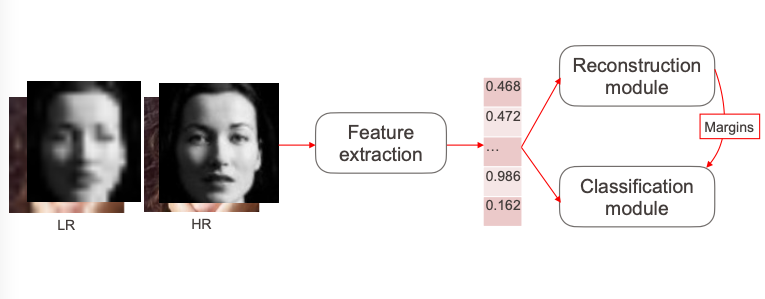
\includegraphics[width=\textwidth]{derivenet.png}
    \caption{DeriveNet}
    \label{fig:derivenet}
\end{figure}

\section{Low Resolution Face Recognition Datasets and Evaluation Protocols}

For further experiments and evaluation of the quality of recognition of face recognition algorithms, 3 datasets and their corresponding protocols were selected. In this chapter, these datasets containing images of faces in low quality, both synthesized and obtained by surveillance  cameras in different shooting conditions, are considered.
\subsection{LFW}
One of the most common datasets for assessing the accuracy of face recognition is Labeled Faces in the Wild (LFW) \cite{lfw}. The protocol involves matching pairs of faces. It contains over 13000 images of 1680 identities. For the LFW dataset, cross-resolution face verification accuracy is calculated for such image sizes as (7.7), (14, 14), (28, 28), (56, 56), (112, 112). Image examples in resolutions used for cross-resolution verification are presented at the \ref{fig:lfw}.

The evaluation protocol is Image Restricted Configuration \cite{lfw}, that is, the pairs of images processed by the algorithm are fixed in advance. The problem to be solved is the verification problem, that is, the binary classification about the belonging of 2 face images to the same person, the problems are described in more detail in the section 6.4 Evaluation. 

\begin{figure}[ht!]
    \centering
    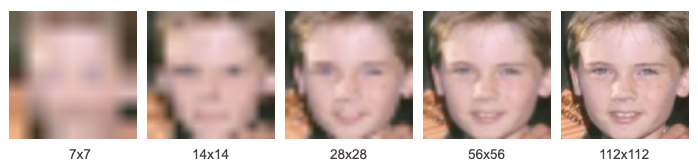
\includegraphics[width=\textwidth]{lfw.png}
    \caption{Example of LFW image and its downsampled variations}
    \label{fig:lfw}
\end{figure}

\subsection{QMUL-SurvFace}
The QMUL-SurvFace \cite{qmul} dataset is used to evaluate the accuracy of low resolution image recognition algorithms. It includes low-resolution images obtained from real-world  conditions, and not through synthesis. Images are characterized by natural  obstacles, such as distractions, changes in cameras conditions, poses, and facial variations. This database contains 463,507 face images of 15,573 identities, however only a part of them is used for testing. As examples, images of different resolutions are presented at \ref{fig:qmul}.

The evaluation protocol includes 2 possible configurations - solving the verification or identification problem, the detailed tasks are described in the section 6.4 Evaluation. For the experiments in this work, the verification task was chosen. As for the previous dataset, the protocol is Image Restricted Configuration \cite{lfw}, that is, the pair lists are fixed in advance. 

\begin{figure}[ht!]
    \centering
    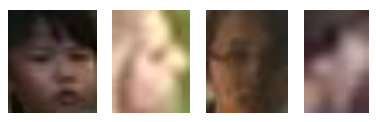
\includegraphics[width=\textwidth]{qmul.png}
    \caption{Example of QMUL-SurvFace images}
    \label{fig:qmul}
\end{figure}

\subsection{SCface}
The SCface \cite{scface} dataset includes images from 3 different surveillance cameras at 3 different distances. Each camera captures images at a low resolution, but variations in  distance produce images of varying degrees of resolution. Thus, the dataset includes 3 possibilities for assessing the quality of recognition, depending on the distance of the location of the camera on which the shooting was made. Also the dataset includes cameras for Day Time and Night Time shooting. The examples for both are presented for all 3 distances at \ref{fig:scface_day} and \ref{fig:scface_night}. However, for the experiments only the Day Time protocol images are used. 

For each protocol, there are 2 datasets dev and eval containing 44 and 43 personalities, respectively. Each identity also has a high-resolution template frontal image as a gallery image against which it will later be compared for identification. The resulting images are characterized by a high quality variability, which makes it possible to evaluate the cross resolution  FR. This dataset is used in the evaluation of such low-resolution image recognition algorithms as \cite{25}.

\begin{figure}[ht!]
    \centering
    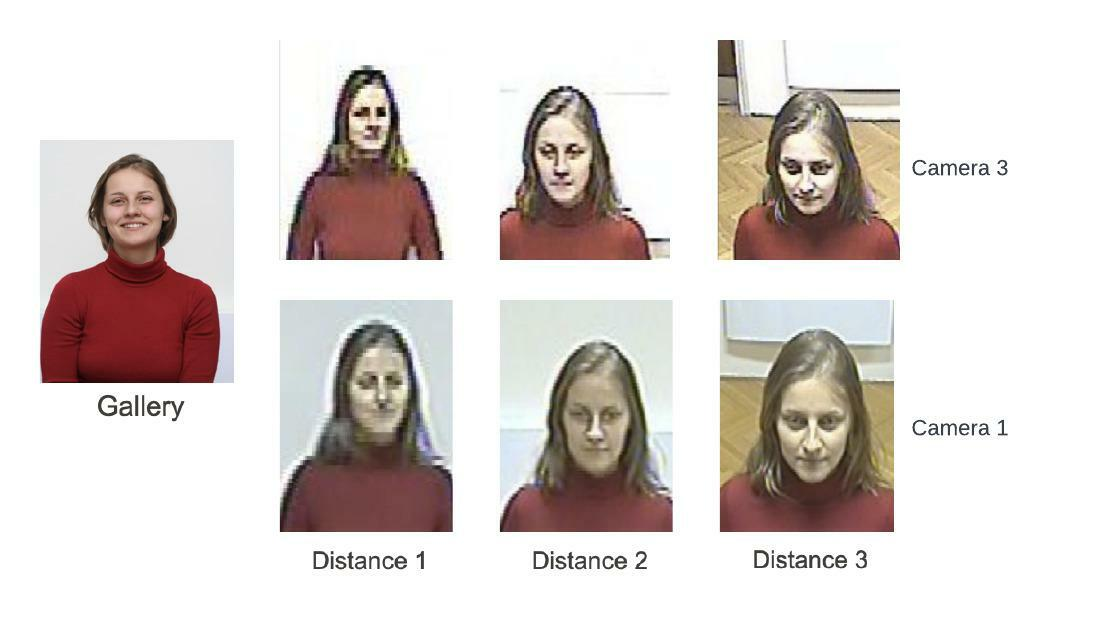
\includegraphics[width=\textwidth]{scface_day.jpeg}
    \caption{Examples of SCface images: DayTime protocol, distance 1, 2, 3}
    \label{fig:scface_day}
\end{figure}

\begin{figure}[ht!]
    \centering
    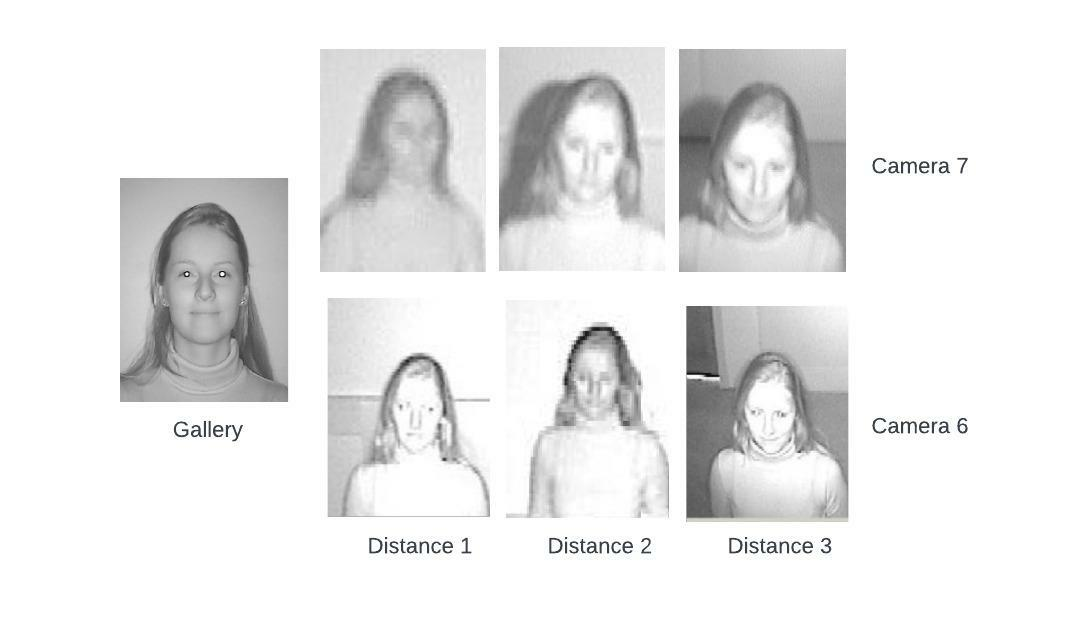
\includegraphics[width=\textwidth]{scface_night.jpeg}
    \caption{Examples of SCface images: NightTime protocol, distance 1, 2, 3}
    \label{fig:scface_night}
\end{figure}

\section{Implemented Low Resolution Face Recognition Methods}
Some of the above methods for solving the LRFR problem were implemented as part of this work. They can be divided into 2 groups: methods that are based on high-resolution FR algorithms and fine-tuning methods. 

\subsection{Adapting High Resolution Face Recognition Methods}
\subsubsection{Cross Resolution Batch Training}
In order to adapt existing methods that have shown better results in high resolution FR, there are different techniques, one of which is Cross Resolution Batch Training \cite{Susceptibility}. The idea is that each neural network processed by the dataset consists of half of the high quality images, and the other half contains downsampled images of the same dataset, but not included in the first set of high resolution images. The workflow is shown at \ref{fig:cross_resolution}. In the experiments, the downsampled images are obtained by resizing the image from (112, 112) to (16, 16) and then interpolated to the original size. 

\begin{figure}[ht!]
    \centering
    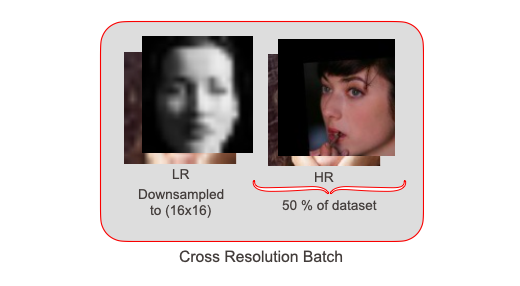
\includegraphics[width=\textwidth]{CR_batch.png}
    \caption{Cross Resolution Batch Training}
    \label{fig:cross_resolution}
\end{figure}

\subsubsection{Softmax-based Loss functions} 
These high-resolution FR algorithms are taken: CosFace \cite{cosface}, SphereFace \cite{sphereface}, ArcFace \cite{arcface}. To describe their implementation, Softmax \cite{softmax} can be written as follows:

$$L = - \log \frac {\exp(f(\theta_{y_i}, m))} {\exp(f(\theta_{y_i}, m)) + \sum_{j \neq y_i}^n{\exp(s \cos \theta_j})}.$$

Then all methods differ in the internal function $f$. For each method they are presented below. This formulation, also used in AdaFace \cite{adaface}, will be used later to describe other algorithms. 

SphereFace \cite{sphereface}: 
\begin{equation*}
f(\theta_j, m) =
\begin{cases}
    s \cos(m\theta_j), & j=y_i;\\
    s \cos(\theta_j), & j \neq y_i.
\end{cases}
\end{equation*}

CosFace \cite{cosface}: 
\begin{equation*}
f(\theta_j, m) =
\begin{cases}
    s (\cos\theta_j - m), & j=y_i;\\
    s \cos(\theta_j), & j \neq y_i.
\end{cases}
\end{equation*}

ArcFace \cite{arcface}: 
\begin{equation*}
f(\theta_j, m) =
\begin{cases}
     s \cos(\theta_j + m), & j=y_i;\\
     s \cos(\theta_j), & j \neq y_i.
\end{cases}
\end{equation*}

\subsubsection{Experiments}
All experiments correspond to the training settings described in section 6.3 Training Settings. The average accuracy for cross-validation on 10 folds was taken as an estimate of the metric.  The evaluation of algorithms based on the 3 datasets protocols described in section 6.4 Evaluation. Results are shown in Table \ref{t1}. 

\begin{table}[ht!]
\begin{center}
\begin{tabular}{||c | c c c||} 
 \hline
 Dataset & CosFace & SphereFace & ArcFace \\ [0.5ex] 
 \hline\hline
 LFW (112x112) & 0.979 & 0.9641 & 0.9773 \\ 
 \hline
  LFW (56x56) & 0.9801 & 0.9625 & 0.97399 \\
 \hline
  LFW (28x28) & 0.9721 & 0.9025 & 0.96933 \\
 \hline
  LFW (14x14) & 0.9266 & 0.7155 & 0.9189 \\
 \hline
  LFW (7x7) & 0.7543 & 0.5926 & 0.74666 \\ 
  \hline
  QMUL-SurvFace & 0.6411 & 0.5953 & 0.6303 \\ 
  \hline
  SCface, dist 1 & 0.6873 & 0.1253 & 0.7349 \\ 
  \hline
  SCface, dist 2 & 0.9336 & 0.3487 & 0.95679 \\ 
  \hline
  SCface, dist 3 & 0.9229 & 0.5654 & 0.9322 \\ [1ex] 
 \hline
\end{tabular}
\caption{Comparison of the accuracy of CosFace, SphereFace and ArcFace obtained at 10 fold cross-validation}
\label{t1}
\end{center}
\end{table}

As a result, we can conclude that the best performance for LFW \cite{lfw}, QMUL-SurvFace \cite{qmul} showed CosFace \cite{cosface}. However, ArcFace \cite{arcface} is slightly worse for these datasets, but shows higher accuracy for SCface \cite{scface}. The SphereFace \cite{sphereface} algorithm showed significantly worse results for all evaluation protocols. Thus, choosing among 3 algorithms, ArcFace \cite{arcface} was the most stable in evaluation. 

\subsection{Finetuning}
The 2 algorithms Octuplet Loss \cite{26} and DeriveNet \cite{derivenet} were taken to solve the LRFR problem by fine-tuning the pre-trained model. 

\subsubsection{Octuplet Loss}
As described in the section 2 Related Work, Octuplet Loss \cite{26} is based on calculating the triplet loss \cite{tripletLoss} of high-resolution images and their downsampled versions. As shown at \ref{fig:octuplet}, Octuplet Loss \cite{26} includes 4 triplet loss components marked with different colors. Thus the formula is: 

$$L = L_{\mathrm{triplet} (T_{hhh})} + L_{\mathrm{triplet} (T_{hll})} + L_{\mathrm{triplet} (T_{lhh})} + L_{\mathrm{triplet} (T_{lll})},$$ 
where $L_{\mathrm{triplet} (T_{hhh})}$ means the triplet loss, and $T_{hhh}, T_{hll}, T_{lhh}, T_{lll}$ mean triplets formed as high resolution (HR) anchor, positive and negative images; HR anchor and low resolution (LR) positive and negative images; LR anchor and HR positive and negative images; and all images are LR, respectively. As the distance in triplet loss the cosine distance is used. 

To test this algorithm, it was necessary to implement a Data Loader for generating triplets, as well as a neural network training function for getting  embeddings of each triplet images.

\subsubsection{DeriveNet} 
The DeriveNet \cite{derivenet} algorithm consists of 2 models: Reconstruction and Classification. The scheme of the algorithm is shown at \ref{fig:derivenet}. A loss function is formulated for each of them: ReCent Loss for Reconstruction module and D-Margin for Classification module, 

$$L_\textrm{D-Margin} = - \log \frac{\exp{\lVert W_{y_i} \rVert \lVert x_i \rVert \cos \theta_{y_i} + D(C_{y_i}, C_j)}}{\sum_{j=1}^C \exp{\lVert W_j \rVert \lVert x_i \rVert \cos \theta_j + D(C_{y_i}, C_j)}},$$ 
where $D$ is the similarity function between 2 classes; 

$$L_\textrm{ReCent} = \lambda ({\lVert \mathrm{HR}_i - g(x_i) \rVert}_2^2 + {\lVert g(x_i) - C_{y_i} \rVert}_2^2,$$
where $g$ refers to the reconstruction module and ${\rm HR_i}$ is the HR image. 

To test this algorithm, it was necessary to implement the modules, their loss functions and the data loader which produces the pairs of images in HR and LR. 

\subsubsection{Experiments}
Arcface \cite{arcface} pretrained is used as the basis for both fine-tuning algorithms in accordance with the settings from the section 6.3 Training Settings with a training sample in high resolution. For fine-tuning, training took place over 6 epochs with settings identical to those described in the sectrion 6.3 Training Settings. The results are presented in Table \ref{t2}.

\begin{table}[ht!]
\begin{center}
\begin{tabular}{||c | c c||} 
 \hline
 Dataset & Octuplet Loss & DeriveNet \\ [0.5ex] 
 \hline\hline
 LFW (112x112) & 0.9208 & 0.9878  \\ 
 \hline
  LFW (56x56) & 0.9211 & 0.9873 \\
 \hline
  LFW (28x28) & 0.9135 & 0.9471  \\
 \hline
  LFW (14x14) & 0.8616  & 0.7103 \\
 \hline
  LFW (7x7) & 0.7375 & 0.5708 \\ 
  \hline
  QMUL-SurvFace & 0.6602 & 0.5618 \\ 
  \hline
  SCface, dist 1 & 0.5095 & 0.346 \\ 
  \hline
  SCface, dist 2 & 0.6296 & 0.8302 \\ 
  \hline
  SCface, dist 3 & 0.4175 & 0.9583 \\ [1ex] 
 \hline
\end{tabular}
\caption{Comparison of the accuracy of Octuplet Loss and DeriveNet obtained at 10 fold cross-validation}
\label{t2} 
\end{center}
\end{table}

As a result, when comparing 2 algorithms, DeriveNet \cite{derivenet} showed the best results for high resolution, and Octuplet Loss \cite{26} for low resolution. However, since for the effectiveness of face recognition with the SCface \cite{scface} dataset protocol, it is also necessary to identify a feature vector from high-quality gallery images, for distances 2 and 3, where the test images of surveillance cameras are characterized by a higher resolution than at distance 1, the DeriveNet\cite{derivenet} algorithm has a higher accuracy.

\section{Proposed Methods}
Recent loss functions for face recognition imply adaptability for fitting hyperparameters \cite{22Ada, 40Ada} , to prevent overfitting \cite{curricularFace} , and to adjust the margin in the loss functions \cite{magface, adaface} .

\subsection{Motivation}
The use of margin-based loss function modifications led to an improvement in the quality of face recognition. One of the state-of-the-art Cross Resolution Face Recognition algorithms, AdaFace \cite{adaface} , proposed the idea of loss function adaptivity to image quality using margin. This method is implemented in the form of an adaptive margin function when approximating the image quality using feature norms.

In order to deal with low resolution images the training methodology of the proposed method is chosen similar to AdaFace \cite{adaface}. Compared to MagFace's \cite{magface} strategy, where high norms (which are easier to recognize) are matched by high margins, AdaFace \cite{adaface} can handle hard-to-find instances, such as low-resolution images. Thus, in order to improve cross resolution face recognition efficiency, a large margin needs to be matched with low quality images.

\subsection{Approach 1}
The main idea of the proposed methods is, in accordance with the articles described in the section 5.1 Motivation, the adaptation of the margin in the loss function based on Softmax \cite{softmax} (in this case, ArcFace \cite{arcface}) depending on the quality of the image. Since the Cross Resolution Patch Training strategy \cite{Susceptibility} described in section 4.1.1 is used for training, images are characterized by 2 resolutions: low and high, so there are 2 cases for the algorithm. For ArcFace \cite{arcface} training, the optimal margin values are from 0.35 to 0.5, so these 2 extreme values will be used to adapt the ArcFace \cite{arcface} to LR face recognition. Accordingly, within the framework of the softmax \cite{softmax} function presented in the form from section 4.1.2, the adaptive margin function implemented in this section can be written as:

\begin{equation*}
f(\theta_j, m) =
\begin{cases}
    s \cos(\theta_j + m), & j=y_i; \\
    s \cos(\theta_j), & j \neq y_i.
\end{cases}
\end{equation*} where $m = 0.35$ if the input is HR and $m=0.5$ otherwise. 

The scheme of the algorithm is shown at \ref{fig:app1}.

\begin{figure}[ht!]
    \centering
    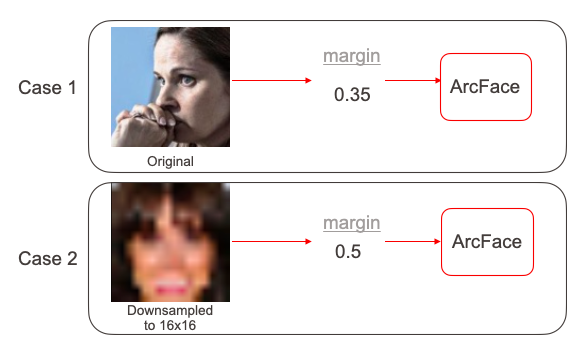
\includegraphics[width=\textwidth]{app1.png}
    \caption{Proposed Method 1}
    \label{fig:app1}
\end{figure}

\subsection{Approach 2}
However in the training dataset there are images of different resolutions \cite{webface}, in order to differentiate them we should use the image quality function. 

\subsubsection{Quality of Image}

Image quality in this case implies the ability to be recognized. Thus, to evaluate it, it is necessary to apply methods that recognize facial features in the image, but do not require much time, as they are used in training. One of the basic methods is based on the discrete representation of the derivative. However, first order derivatives such as Sobel and Prewitt are sensitive to noise \cite{QualityImage2}. The Laplacian operator based on second derivatives does not have such a drawback \cite{QualityImage}. To get the value expressed by 1 number, it is necessary to calculate the metric of the matrix obtained using Laplacian. In this paper, it is proposed to take the average discriminative Laplacian as the image quality metric. To demonstrate the effectiveness of this image quality evaluation function, at \ref{fig:image_quality} there are examples of high and low resolution images for which norms have been calculated.

\begin{figure}[ht!]
    \centering
    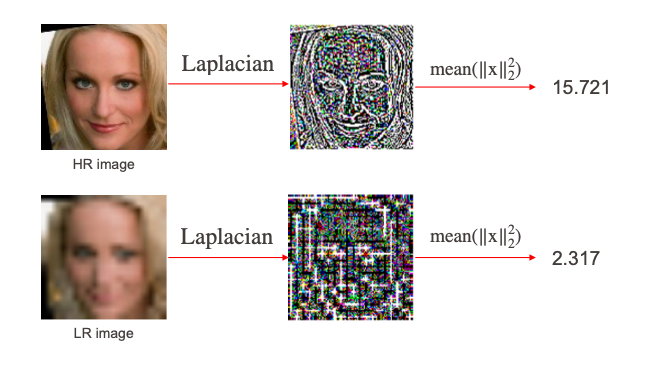
\includegraphics[width=\textwidth]{image_quality.png}
    \caption{Comparison of Image quality using the Laplacian operator}
    \label{fig:image_quality}
\end{figure}

\subsubsection{Definition}
Thus, as the adaptive margin loss function, it is proposed to take the head algorithm based on ArcFace with adapted margins based on average Laplacian for processing low-resolution images. Since a high value of the Laplacian norm indicates a high image quality, it is proposed to take its reciprocal value as a margin. Thus, for low quality images, the margin will be higher. \ref{fig:app2} shows the scheme of the algorithm.

\begin{figure}[ht!]
    \centering
    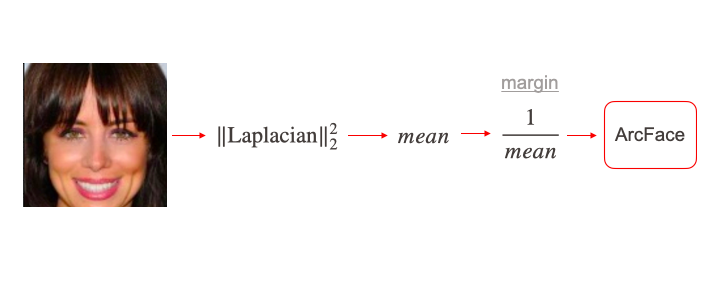
\includegraphics[width=\textwidth]{app2.png}
    \caption{Proposed Method 2}
    \label{fig:app2}
\end{figure}

\subsubsection{Discussion}
But for high resolution images the margin is to low, so in the future it's proposed to modify the function mapping image quality  to margin in such a way that the margin value is bounded by reasonable for ArcFace \cite{arcface} values. For the current approach the accuracy for high resolution is low because of non-convenient margin values.  

\section{Experiments}
\subsection{Training Dataset}
CASIA-WebFace \cite{webface} is chosen as the training dataset. It contains 494,414 images of 10,575 real identities. The database includes images of celebrities' faces.
\subsection{Preprocessing of training data}
The MTCNN \cite{2} algorithm is used to prepare images for both training and testing. In this way the areas of the image containing the face are obtained and aligned. Each image is resized to (112, 112) and normalized. A vertical flip with a probability of 0.5 is added as an augmentation. Half of the dataset is artificially downsampled to a resolution of (16, 16) and restored by linear interpolation to the original size in order to preserve the dimensions of the input data.
\subsection{Training Settings}
ResNet50 is used as the backbone of the neural network. Training is done using the SGD optimizer with the initial learning rate of 0.1 and learning rate step scheduling at 5, 10 and 15 epochs. The scale parameter of head neural network $s$  is equal to 64. Training lasts 18 epochs.
\subsection{Evaluation} 
To test the proposed method, the verification problem is solved for 3 test datasets described in section 3 Low Resolution Face Recognition Dtasets and Evaluation Protocols.

When testing the algorithm, it is necessary to calculate the accuracy of solving the problems of verification and identification of a person from an image. As a test dataset, a set of IDs is presented, including one or more photographs of faces. After applying the trained model to the test dataset, a database of extracted embeddings is formed.

Verification is a 1-to-1 matching process that checks if the face embedding belongs to the ID class. This process is done by calculating the similarity metric between the current embedding and the ID class embedding from the embedding database. If the metric value exceeds a fixed threshold, then the image presented as the current embedding belongs to the ID class.

Identification is a task of matching 1 to N. The input is an image and a set of IDs, the output of the algorithm is the class to which the image belongs or a message that the class is not recognized. Similar to verification, the similarity metric is considered for N presented classes, among which the maximum is selected. If the maximum similarity value exceeds the threshold, then the corresponding ID is the solution to the problem.

\subsection{Analysis}
The comparison is made based on mean accuracy of 10-fold cross validation. The AdaFace \cite{adaface} algorithm is chosen as the state-of-the art algorithm to compare the performance with respect to modern low-resolution face recognition methods. 

\subsubsection{Comparison with the baseline}
This section presents a comparison of the proposed methods with baseline algorithm AdaFace \cite{adaface} in the Table \ref{t3}.

\begin{table}[ht!]
\begin{center}
\begin{tabular}{||c | c c c||} 
 \hline
 Dataset & AdaFace & Approach1 & Approach2 \\ [0.5ex] 
 \hline\hline
 LFW (112x112) & 0.9906 & 0.977 & 0.9623 \\ 
 \hline
  LFW (56x56) & 0.9869 & 0.974 & 0.9645 \\
 \hline
  LFW (28x28) & 0.9685 & 0.969 & 0.9584 \\
 \hline
  LFW (14x14) & 0.6321 & 0.9236 & 0.9138 \\
 \hline
  LFW (7x7) & 0.5653 & 0.7685 & 0.7905 \\ 
  \hline
  QMUL-SurvFace, mean accuracy & 0.5324 & 0.6281 & 0.7125 \\ 
  \hline
  QMUL-SurvFace, std & 0.04875 & 0.02956 & 0.0265 \\  
 \hline
 SCface, dist 1 &  0.50634 & 0.7539 & 0.7492 \\ 
  \hline
  SCface, dist 2 & 0.96913 & 0.9506 & 0.9182 \\ 
  \hline
  SCface, dist 3 & 0.99691 & 0.9491 & 0.8104 \\ [1ex]
  \hline
\end{tabular}
\caption{Comparison of the accuracy of AdaFace and 2 proposed methods obtained at 10 fold cross-validation}
\label{t3} 
\end{center}
\end{table}

Based on the results obtained when testing the AdaFace \cite{adaface} baseline and the proposed methods, we can conclude that the proposed algorithms are applicable to solving the LR face recognition problem, since they outperformed AdaFace \cite{adaface} in these tests when evaluating low-resolution images. However, in high resolution and when evaluating SCface \cite{scface}, where it is necessary to process high-resolution images from the gallery, AdaFace \cite{adaface} showed the best accuracy.

\subsubsection{Comparison of all implemented methods}
For clarity, the \ref{t4} is also presented containing the accuracy values for the test protocols of all the methods implemented in the work.

\begin{table}[ht!]
\begin{center}
\resizebox{\columnwidth}{!}{\begin{tabular}{||c | c c c c c c c c||} 
 \hline
 Dataset & CosFace & SphereFace & ArcFace & Octuplet Loss & DeriveNet & AdaFace & Approach1 & Approach2 \\ [0.5ex] 
 \hline\hline
 LFW (112x112) & 0.979 & 0.9641 & 0.9773 & 0.9208 & 0.9878 & 0.9906 & 0.977 & 0.9623  \\ 
 \hline
  LFW (56x56) & 0.9801 & 0.9625 & 0.97399 & 0.9211 & 0.9873 & 0.9869 & 0.974 & 0.9645  \\
 \hline
  LFW (28x28) & 0.9721 & 0.9025 & 0.96933 & 0.9135 & 0.9471 & 0.9685 & 0.969 & 0.9584  \\
 \hline
  LFW (14x14) & 0.9266 & 0.7155 & 0.9189 & 0.8616 & 0.7103 & 0.6321 & 0.9236 & 0.9138 \\
 \hline
  LFW (7x7) & 0.7543 & 0.5926 & 0.74666 & 0.7375 & 0.5708 & 0.5653 & 0.7685 & 0.7905 \\ 
  \hline
  QMUL-SurvFace & 0.6411 & 0.5953 & 0.6303 & 0.6602 & 0.5618 & 0.5324 & 0.6281 & 0.7125 \\ 
  \hline
  SCface, dist 1 & 0.6873 & 0.1253 & 0.7349 & 0.5095 & 0.346 & 0.50634 & 0.7539 & 0.7492 \\ 
  \hline
  SCface, dist 2 & 0.9336 & 0.3487 & 0.95679 & 0.6296 & 0.8302 & 0.96913 & 0.9506 & 0.9182 \\ 
  \hline
  SCface, dist 3 & 0.9229 & 0.5654 & 0.9322 & 0.4175 & 0.9583 & 0.99691 & 0.9491 & 0.8104 \\ [1ex] 
 \hline
\end{tabular}}
\caption{Comparison of the accuracy of all implemented methods and AdaFace obtained at 10 fold cross-validation}
\label{t4}
\end{center}
\end{table}
\newpage
\section{Conclusion}
In this work, the problem of low-resolution facial recognition and methods of its solution based on deep training were studied. For the implementation of some of these methods, a face recognition pipeline for deep learning based on the existing solution was implemented. In addition, low-resolution datasets were studied: LFW, QMUL-SurvFace, SCface, for each dataset the evaluation protocol was implemented. In the course of the project, high-resolution facial recognition methods were implemented: CosFace, SphereFace, ArcFace, and adapted to solve the low-resolution facial recognition problem using the Cross Resolution Batch Training algorithm. Also algorithms for fine-tuning facial recognition model were implemented: OctupletLos, DeriveNet. Based on the studied articles and the trend towards margin adaptation in software-based loss functions, two methods were proposed, one of which sets two fixed margin values depending on whether the image is of high or low quality being processed, and the second evaluates the image quality with the help of Laplacian operator. All implemented methods were tested based on low resolution image datasets. To assess the quality of the proposed methods, the AdaFace algorithm was chosen as a baseline, which is state-of-the-art in Cross Resolution Face Recognition. As a result of the evaluation, algorithms showed accuracy higher than those of AdaFace in low resolution images. 

\newpage

\addcontentsline{toc}{section}{References}

\bibliographystyle{plain}
\bibliography{bibliography}

% \begin{thebibliography}{99}

% \bibitem{QualityImage}
% E. A. Ru \'{a}, J. E. L. A. Castro, and C. G. Mateo, “Quality- Based Score Normalization and Frame Selection for Video- Based Person Authentication,” in Biometrics and Identity Management (BioID), vol. 5372, Springer Berlin / Heidel- berg, 2008, pp. 1–9, ISBN: 978-3-540-89990-7 978-3-540- 89991-4.

% % \bibitem{}

% \end{thebibliography}


\end{document}

